% Options for packages loaded elsewhere
\PassOptionsToPackage{unicode}{hyperref}
\PassOptionsToPackage{hyphens}{url}
\PassOptionsToPackage{dvipsnames,svgnames,x11names}{xcolor}
%
\documentclass[
  letterpaper,
  DIV=11,
  numbers=noendperiod]{scrartcl}

\usepackage{amsmath,amssymb}
\usepackage{iftex}
\ifPDFTeX
  \usepackage[T1]{fontenc}
  \usepackage[utf8]{inputenc}
  \usepackage{textcomp} % provide euro and other symbols
\else % if luatex or xetex
  \usepackage{unicode-math}
  \defaultfontfeatures{Scale=MatchLowercase}
  \defaultfontfeatures[\rmfamily]{Ligatures=TeX,Scale=1}
\fi
\usepackage{lmodern}
\ifPDFTeX\else  
    % xetex/luatex font selection
\fi
% Use upquote if available, for straight quotes in verbatim environments
\IfFileExists{upquote.sty}{\usepackage{upquote}}{}
\IfFileExists{microtype.sty}{% use microtype if available
  \usepackage[]{microtype}
  \UseMicrotypeSet[protrusion]{basicmath} % disable protrusion for tt fonts
}{}
\makeatletter
\@ifundefined{KOMAClassName}{% if non-KOMA class
  \IfFileExists{parskip.sty}{%
    \usepackage{parskip}
  }{% else
    \setlength{\parindent}{0pt}
    \setlength{\parskip}{6pt plus 2pt minus 1pt}}
}{% if KOMA class
  \KOMAoptions{parskip=half}}
\makeatother
\usepackage{xcolor}
\setlength{\emergencystretch}{3em} % prevent overfull lines
\setcounter{secnumdepth}{5}
% Make \paragraph and \subparagraph free-standing
\ifx\paragraph\undefined\else
  \let\oldparagraph\paragraph
  \renewcommand{\paragraph}[1]{\oldparagraph{#1}\mbox{}}
\fi
\ifx\subparagraph\undefined\else
  \let\oldsubparagraph\subparagraph
  \renewcommand{\subparagraph}[1]{\oldsubparagraph{#1}\mbox{}}
\fi

\usepackage{color}
\usepackage{fancyvrb}
\newcommand{\VerbBar}{|}
\newcommand{\VERB}{\Verb[commandchars=\\\{\}]}
\DefineVerbatimEnvironment{Highlighting}{Verbatim}{commandchars=\\\{\}}
% Add ',fontsize=\small' for more characters per line
\usepackage{framed}
\definecolor{shadecolor}{RGB}{241,243,245}
\newenvironment{Shaded}{\begin{snugshade}}{\end{snugshade}}
\newcommand{\AlertTok}[1]{\textcolor[rgb]{0.68,0.00,0.00}{#1}}
\newcommand{\AnnotationTok}[1]{\textcolor[rgb]{0.37,0.37,0.37}{#1}}
\newcommand{\AttributeTok}[1]{\textcolor[rgb]{0.40,0.45,0.13}{#1}}
\newcommand{\BaseNTok}[1]{\textcolor[rgb]{0.68,0.00,0.00}{#1}}
\newcommand{\BuiltInTok}[1]{\textcolor[rgb]{0.00,0.23,0.31}{#1}}
\newcommand{\CharTok}[1]{\textcolor[rgb]{0.13,0.47,0.30}{#1}}
\newcommand{\CommentTok}[1]{\textcolor[rgb]{0.37,0.37,0.37}{#1}}
\newcommand{\CommentVarTok}[1]{\textcolor[rgb]{0.37,0.37,0.37}{\textit{#1}}}
\newcommand{\ConstantTok}[1]{\textcolor[rgb]{0.56,0.35,0.01}{#1}}
\newcommand{\ControlFlowTok}[1]{\textcolor[rgb]{0.00,0.23,0.31}{#1}}
\newcommand{\DataTypeTok}[1]{\textcolor[rgb]{0.68,0.00,0.00}{#1}}
\newcommand{\DecValTok}[1]{\textcolor[rgb]{0.68,0.00,0.00}{#1}}
\newcommand{\DocumentationTok}[1]{\textcolor[rgb]{0.37,0.37,0.37}{\textit{#1}}}
\newcommand{\ErrorTok}[1]{\textcolor[rgb]{0.68,0.00,0.00}{#1}}
\newcommand{\ExtensionTok}[1]{\textcolor[rgb]{0.00,0.23,0.31}{#1}}
\newcommand{\FloatTok}[1]{\textcolor[rgb]{0.68,0.00,0.00}{#1}}
\newcommand{\FunctionTok}[1]{\textcolor[rgb]{0.28,0.35,0.67}{#1}}
\newcommand{\ImportTok}[1]{\textcolor[rgb]{0.00,0.46,0.62}{#1}}
\newcommand{\InformationTok}[1]{\textcolor[rgb]{0.37,0.37,0.37}{#1}}
\newcommand{\KeywordTok}[1]{\textcolor[rgb]{0.00,0.23,0.31}{#1}}
\newcommand{\NormalTok}[1]{\textcolor[rgb]{0.00,0.23,0.31}{#1}}
\newcommand{\OperatorTok}[1]{\textcolor[rgb]{0.37,0.37,0.37}{#1}}
\newcommand{\OtherTok}[1]{\textcolor[rgb]{0.00,0.23,0.31}{#1}}
\newcommand{\PreprocessorTok}[1]{\textcolor[rgb]{0.68,0.00,0.00}{#1}}
\newcommand{\RegionMarkerTok}[1]{\textcolor[rgb]{0.00,0.23,0.31}{#1}}
\newcommand{\SpecialCharTok}[1]{\textcolor[rgb]{0.37,0.37,0.37}{#1}}
\newcommand{\SpecialStringTok}[1]{\textcolor[rgb]{0.13,0.47,0.30}{#1}}
\newcommand{\StringTok}[1]{\textcolor[rgb]{0.13,0.47,0.30}{#1}}
\newcommand{\VariableTok}[1]{\textcolor[rgb]{0.07,0.07,0.07}{#1}}
\newcommand{\VerbatimStringTok}[1]{\textcolor[rgb]{0.13,0.47,0.30}{#1}}
\newcommand{\WarningTok}[1]{\textcolor[rgb]{0.37,0.37,0.37}{\textit{#1}}}

\providecommand{\tightlist}{%
  \setlength{\itemsep}{0pt}\setlength{\parskip}{0pt}}\usepackage{longtable,booktabs,array}
\usepackage{calc} % for calculating minipage widths
% Correct order of tables after \paragraph or \subparagraph
\usepackage{etoolbox}
\makeatletter
\patchcmd\longtable{\par}{\if@noskipsec\mbox{}\fi\par}{}{}
\makeatother
% Allow footnotes in longtable head/foot
\IfFileExists{footnotehyper.sty}{\usepackage{footnotehyper}}{\usepackage{footnote}}
\makesavenoteenv{longtable}
\usepackage{graphicx}
\makeatletter
\def\maxwidth{\ifdim\Gin@nat@width>\linewidth\linewidth\else\Gin@nat@width\fi}
\def\maxheight{\ifdim\Gin@nat@height>\textheight\textheight\else\Gin@nat@height\fi}
\makeatother
% Scale images if necessary, so that they will not overflow the page
% margins by default, and it is still possible to overwrite the defaults
% using explicit options in \includegraphics[width, height, ...]{}
\setkeys{Gin}{width=\maxwidth,height=\maxheight,keepaspectratio}
% Set default figure placement to htbp
\makeatletter
\def\fps@figure{htbp}
\makeatother
% definitions for citeproc citations
\NewDocumentCommand\citeproctext{}{}
\NewDocumentCommand\citeproc{mm}{%
  \begingroup\def\citeproctext{#2}\cite{#1}\endgroup}
\makeatletter
 % allow citations to break across lines
 \let\@cite@ofmt\@firstofone
 % avoid brackets around text for \cite:
 \def\@biblabel#1{}
 \def\@cite#1#2{{#1\if@tempswa , #2\fi}}
\makeatother
\newlength{\cslhangindent}
\setlength{\cslhangindent}{1.5em}
\newlength{\csllabelwidth}
\setlength{\csllabelwidth}{3em}
\newenvironment{CSLReferences}[2] % #1 hanging-indent, #2 entry-spacing
 {\begin{list}{}{%
  \setlength{\itemindent}{0pt}
  \setlength{\leftmargin}{0pt}
  \setlength{\parsep}{0pt}
  % turn on hanging indent if param 1 is 1
  \ifodd #1
   \setlength{\leftmargin}{\cslhangindent}
   \setlength{\itemindent}{-1\cslhangindent}
  \fi
  % set entry spacing
  \setlength{\itemsep}{#2\baselineskip}}}
 {\end{list}}
\usepackage{calc}
\newcommand{\CSLBlock}[1]{\hfill\break\parbox[t]{\linewidth}{\strut\ignorespaces#1\strut}}
\newcommand{\CSLLeftMargin}[1]{\parbox[t]{\csllabelwidth}{\strut#1\strut}}
\newcommand{\CSLRightInline}[1]{\parbox[t]{\linewidth - \csllabelwidth}{\strut#1\strut}}
\newcommand{\CSLIndent}[1]{\hspace{\cslhangindent}#1}

\KOMAoption{captions}{tableheading}
\makeatletter
\@ifpackageloaded{caption}{}{\usepackage{caption}}
\AtBeginDocument{%
\ifdefined\contentsname
  \renewcommand*\contentsname{Table of contents}
\else
  \newcommand\contentsname{Table of contents}
\fi
\ifdefined\listfigurename
  \renewcommand*\listfigurename{List of Figures}
\else
  \newcommand\listfigurename{List of Figures}
\fi
\ifdefined\listtablename
  \renewcommand*\listtablename{List of Tables}
\else
  \newcommand\listtablename{List of Tables}
\fi
\ifdefined\figurename
  \renewcommand*\figurename{Figure}
\else
  \newcommand\figurename{Figure}
\fi
\ifdefined\tablename
  \renewcommand*\tablename{Table}
\else
  \newcommand\tablename{Table}
\fi
}
\@ifpackageloaded{float}{}{\usepackage{float}}
\floatstyle{ruled}
\@ifundefined{c@chapter}{\newfloat{codelisting}{h}{lop}}{\newfloat{codelisting}{h}{lop}[chapter]}
\floatname{codelisting}{Listing}
\newcommand*\listoflistings{\listof{codelisting}{List of Listings}}
\makeatother
\makeatletter
\makeatother
\makeatletter
\@ifpackageloaded{caption}{}{\usepackage{caption}}
\@ifpackageloaded{subcaption}{}{\usepackage{subcaption}}
\makeatother
\ifLuaTeX
  \usepackage{selnolig}  % disable illegal ligatures
\fi
\usepackage{bookmark}

\IfFileExists{xurl.sty}{\usepackage{xurl}}{} % add URL line breaks if available
\urlstyle{same} % disable monospaced font for URLs
\hypersetup{
  pdftitle={Variation in thermal pressures and resource availability drives disease dynamics},
  colorlinks=true,
  linkcolor={blue},
  filecolor={Maroon},
  citecolor={Blue},
  urlcolor={Blue},
  pdfcreator={LaTeX via pandoc}}

\title{Variation in thermal pressures and resource availability drives
disease dynamics}
\author{Cole Brookson \and David Vasseur}
\date{}

\begin{document}
\maketitle

\renewcommand*\contentsname{Table of contents}
{
\hypersetup{linkcolor=}
\setcounter{tocdepth}{3}
\tableofcontents
}
\subsection{Model}\label{model}

Vinton and Vasseur (2022) provide a basic model for
temperature-dependent consumer-resource dynamics with a chemostat model
of resource, \(R\), supply, given by

\begin{equation}
\label{eq:resource-growth}
\frac{dR}{dt} = D(S-R) - f(R,T)C,
\end{equation}

where there is an inflow density \(S\) and an outflow rate \(D\) and
\(f(R,T)\) i the functional response of \(R\) with respect to
temperature \(T\). The biomass change of the consumer \(C\) is given by

\begin{equation}
\label{eq:consumer-growth}
\frac{dC}{dt} = (1 - \delta)f(R,T) - m(T)C,
\end{equation}

where \((1-\delta)\) is the consumption efficiency (denoted as a
fraction), and \(m\) is the rate of respiration. We assume a
Boltzmann-Arrhenius relationship and approximate that function \(m(T)\)
with

\begin{equation}
\label{eq:respiration-rate}
m(T) = m_ae^{m_bT} + m_c,
\end{equation}

with \(m_a\), \(m_b\) and \(m_c\) all \(>0\). The functional response is
a standard type II, with attack rate \(a\), handling rate \((1/h)\), but
re-state according to the Michaelis-Menten form of

\begin{equation}
\label{eq:functional-response}
f(R,T) = I_{max}(T) \times \frac{R}{R + R_{\text{half}}},
\end{equation}

and \(I_{max}T\) is the maximum uptake rate which we state as equivalent
to the handling rate \(I_{max}T \equiv 1/h\), and then the
half-saturation density is made equivalnt via
\(R_{\text{half}} \equiv \frac{1}{a \times h}\). Note that the resource
saturation is reached by \(R / (R_{\text{half}} + R)\), which is
independent of \(I_{max}\). Last,

\begin{equation}
\label{eq:i-max}
I_{max}(T) = e^{-(T-T_I)^2\gamma},
\end{equation}

is the equation governing the relationship with temperature, where
\(T_I\) is the optimum temperature for consumption, and \(\gamma\) is
the breadth of response.

\subsubsection{Equilibrium Solutions}\label{equilibrium-solutions}

Vinton and Vasseur (2022) showed that there is a coexistence equilibrium
solution where

\begin{equation}
\label{eq:r-equil}
R_e = \frac{m R_\text{half}}{(1-\delta)I_{max}(T) - m},
\end{equation}

and

\begin{equation}
\label{eq:c-equil}
C_e = \frac{D(S-R_e)(R_e - R_\text{half})}{I_{max}(T)R_e},
\end{equation}

\subsubsection{Brute-force Computation}\label{brute-force-computation}

We use the standard set of model parameters for the chemostat dynamics,
\(R_\text{half} = 2, T_I = 25, \gamma = 150, m_a = 0.01, m_b = 0.1, m_c = 0.05, D = 1, S = 1\).

With these values, we set up a brute-force computation that draws values
of R

Here's a single run for R:

\begin{Shaded}
\begin{Highlighting}[]
\CommentTok{\# Load the deSolve package}
\FunctionTok{library}\NormalTok{(deSolve)}
\FunctionTok{library}\NormalTok{(ggplot2)}
\FunctionTok{library}\NormalTok{(magrittr)}
\FunctionTok{library}\NormalTok{(dplyr)}
\end{Highlighting}
\end{Shaded}

\begin{Shaded}
\begin{Highlighting}[]
\CommentTok{\# Define the differential equations}
\NormalTok{consumer\_resource\_model }\OtherTok{\textless{}{-}} \ControlFlowTok{function}\NormalTok{(time, state, parameters) \{}
\NormalTok{    R }\OtherTok{\textless{}{-}}\NormalTok{ state[}\DecValTok{1}\NormalTok{]}
\NormalTok{    C }\OtherTok{\textless{}{-}}\NormalTok{ state[}\DecValTok{2}\NormalTok{]}
\NormalTok{    T }\OtherTok{\textless{}{-}}\NormalTok{ parameters[}\StringTok{"T"}\NormalTok{]}
\NormalTok{    D }\OtherTok{\textless{}{-}}\NormalTok{ parameters[}\StringTok{"D"}\NormalTok{]}
\NormalTok{    S }\OtherTok{\textless{}{-}}\NormalTok{ parameters[}\StringTok{"S"}\NormalTok{]}
\NormalTok{    delta }\OtherTok{\textless{}{-}}\NormalTok{ parameters[}\StringTok{"delta"}\NormalTok{]}
\NormalTok{    m\_a }\OtherTok{\textless{}{-}}\NormalTok{ parameters[}\StringTok{"m\_a"}\NormalTok{]}
\NormalTok{    m\_b }\OtherTok{\textless{}{-}}\NormalTok{ parameters[}\StringTok{"m\_b"}\NormalTok{]}
\NormalTok{    m\_c }\OtherTok{\textless{}{-}}\NormalTok{ parameters[}\StringTok{"m\_c"}\NormalTok{]}
\NormalTok{    a }\OtherTok{\textless{}{-}}\NormalTok{ parameters[}\StringTok{"a"}\NormalTok{]}
\NormalTok{    h }\OtherTok{\textless{}{-}}\NormalTok{ parameters[}\StringTok{"h"}\NormalTok{]}
\NormalTok{    e }\OtherTok{\textless{}{-}}\NormalTok{ parameters[}\StringTok{"e"}\NormalTok{]}
\NormalTok{    gamma }\OtherTok{\textless{}{-}}\NormalTok{ parameters[}\StringTok{"gamma"}\NormalTok{]}
\NormalTok{    T\_I }\OtherTok{\textless{}{-}}\NormalTok{ parameters[}\StringTok{"T\_I"}\NormalTok{]}
\NormalTok{    R\_half }\OtherTok{\textless{}{-}}\NormalTok{ parameters[}\StringTok{"R\_half"}\NormalTok{]}

    \CommentTok{\# Functional response f(R, T)}
\NormalTok{    I\_max\_T }\OtherTok{\textless{}{-}} \FunctionTok{exp}\NormalTok{(}\SpecialCharTok{{-}}\NormalTok{(T }\SpecialCharTok{{-}}\NormalTok{ T\_I)}\SpecialCharTok{\^{}}\DecValTok{2} \SpecialCharTok{*}\NormalTok{ gamma)}
\NormalTok{    f\_R\_T }\OtherTok{\textless{}{-}}\NormalTok{ I\_max\_T }\SpecialCharTok{*}\NormalTok{ R }\SpecialCharTok{/}\NormalTok{ (R }\SpecialCharTok{+}\NormalTok{ R\_half)}

    \CommentTok{\# Respiration rate m(T)}
\NormalTok{    m\_T }\OtherTok{\textless{}{-}}\NormalTok{ m\_a }\SpecialCharTok{*} \FunctionTok{exp}\NormalTok{(m\_b }\SpecialCharTok{*}\NormalTok{ T) }\SpecialCharTok{+}\NormalTok{ m\_c}

    \CommentTok{\# Differential equations}
\NormalTok{    dR\_dt }\OtherTok{\textless{}{-}}\NormalTok{ D }\SpecialCharTok{*}\NormalTok{ (S }\SpecialCharTok{{-}}\NormalTok{ R) }\SpecialCharTok{{-}}\NormalTok{ f\_R\_T }\SpecialCharTok{*}\NormalTok{ C}
\NormalTok{    dC\_dt }\OtherTok{\textless{}{-}}\NormalTok{ (}\DecValTok{1} \SpecialCharTok{{-}}\NormalTok{ delta) }\SpecialCharTok{*}\NormalTok{ f\_R\_T }\SpecialCharTok{{-}}\NormalTok{ m\_T }\SpecialCharTok{*}\NormalTok{ C}

    \FunctionTok{return}\NormalTok{(}\FunctionTok{list}\NormalTok{(}\FunctionTok{c}\NormalTok{(dR\_dt, dC\_dt)))}
\NormalTok{\}}

\CommentTok{\# Define the parameters}
\NormalTok{parameters }\OtherTok{\textless{}{-}} \FunctionTok{c}\NormalTok{(}
    \AttributeTok{T =} \FunctionTok{rnorm}\NormalTok{(}\DecValTok{1}\NormalTok{, }\AttributeTok{mean =} \DecValTok{25}\NormalTok{, }\AttributeTok{sd =} \DecValTok{1}\NormalTok{), }\CommentTok{\# Random normal temperature}
    \AttributeTok{D =} \DecValTok{1}\NormalTok{, }\CommentTok{\# Outflow rate}
    \AttributeTok{S =} \DecValTok{2}\NormalTok{, }\CommentTok{\# Inflow resource density}
    \AttributeTok{delta =} \FloatTok{0.2}\NormalTok{, }\CommentTok{\# Consumption efficiency}
    \AttributeTok{e =} \FloatTok{0.5}\NormalTok{,}
    \AttributeTok{m\_a =} \FloatTok{0.01}\NormalTok{,}
    \AttributeTok{m\_b =} \FloatTok{0.1}\NormalTok{,}
    \AttributeTok{m\_c =} \FloatTok{0.05}\NormalTok{,}
    \AttributeTok{a =} \FloatTok{0.5}\NormalTok{, }\CommentTok{\# Attack rate}
    \AttributeTok{h =} \FloatTok{0.1}\NormalTok{, }\CommentTok{\# Handling rate}
    \AttributeTok{gamma =} \DecValTok{150}\NormalTok{, }\CommentTok{\# Breadth of response}
    \AttributeTok{T\_I =} \DecValTok{25}\NormalTok{, }\CommentTok{\# Optimum temperature for consumption}
    \AttributeTok{R\_half =} \FloatTok{0.5} \CommentTok{\# Half{-}saturation density}
\NormalTok{)}

\CommentTok{\# Define initial conditions for R and C}
\NormalTok{state }\OtherTok{\textless{}{-}} \FunctionTok{c}\NormalTok{(}\AttributeTok{R =} \FloatTok{0.2}\NormalTok{, }\AttributeTok{C =} \FloatTok{0.5}\NormalTok{)}

\CommentTok{\# Set time points for the simulation}
\NormalTok{times }\OtherTok{\textless{}{-}} \FunctionTok{seq}\NormalTok{(}\DecValTok{0}\NormalTok{, }\DecValTok{100}\NormalTok{, }\AttributeTok{by =} \FloatTok{0.1}\NormalTok{)}

\CommentTok{\# Run the simulation using deSolve\textquotesingle{}s ode function}
\NormalTok{output }\OtherTok{\textless{}{-}} \FunctionTok{data.frame}\NormalTok{(deSolve}\SpecialCharTok{::}\FunctionTok{ode}\NormalTok{(}
    \AttributeTok{y =}\NormalTok{ state, }\AttributeTok{times =}\NormalTok{ times,}
    \AttributeTok{func =}\NormalTok{ consumer\_resource\_model,}
    \AttributeTok{parms =}\NormalTok{ parameters}
\NormalTok{)) }\SpecialCharTok{|\textgreater{}}
\NormalTok{    tidyr}\SpecialCharTok{::}\FunctionTok{pivot\_longer}\NormalTok{(}
        \AttributeTok{cols =} \FunctionTok{c}\NormalTok{(R, C),}
        \AttributeTok{names\_to =} \StringTok{"spp"}
\NormalTok{    )}


\CommentTok{\# Plot the results}
\NormalTok{ggplot2}\SpecialCharTok{::}\FunctionTok{ggplot}\NormalTok{(}
    \AttributeTok{data =}\NormalTok{ output}
\NormalTok{) }\SpecialCharTok{+}
    \FunctionTok{geom\_line}\NormalTok{(}\FunctionTok{aes}\NormalTok{(}\AttributeTok{x =}\NormalTok{ time, }\AttributeTok{y =}\NormalTok{ value, }\AttributeTok{colour =}\NormalTok{ spp)) }\SpecialCharTok{+}
    \FunctionTok{theme\_bw}\NormalTok{() }\SpecialCharTok{+}
    \FunctionTok{theme}\NormalTok{(}
        \AttributeTok{text =} \FunctionTok{element\_text}\NormalTok{(}\AttributeTok{size =} \DecValTok{18}\NormalTok{),}
        \AttributeTok{panel.grid.major =} \FunctionTok{element\_blank}\NormalTok{(),}
        \AttributeTok{panel.grid.minor =} \FunctionTok{element\_blank}\NormalTok{(),}
        \AttributeTok{strip.background =} \FunctionTok{element\_blank}\NormalTok{()}
\NormalTok{    ) }\SpecialCharTok{+}
    \FunctionTok{labs}\NormalTok{(}\AttributeTok{x =} \StringTok{"Time"}\NormalTok{, }\AttributeTok{y =} \StringTok{"Density"}\NormalTok{)}
\end{Highlighting}
\end{Shaded}

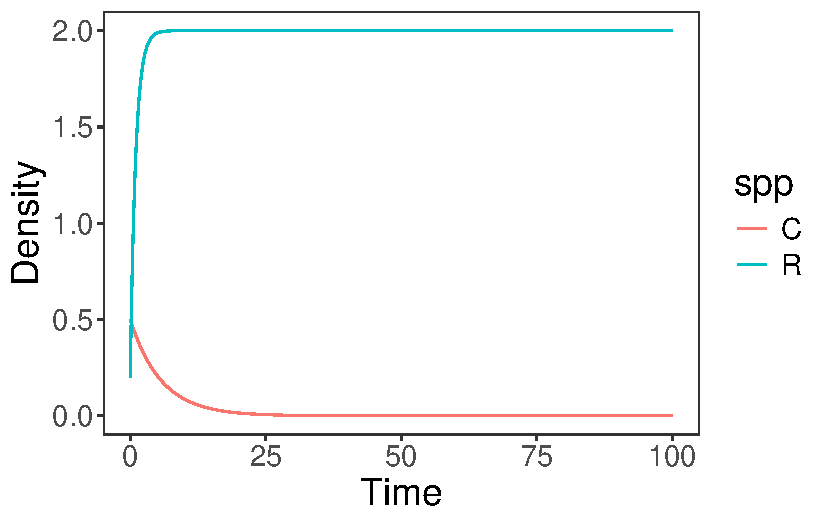
\includegraphics{index_files/figure-pdf/unnamed-chunk-1-1.pdf}

\textsubscript{Source:
\href{https://colebrookson.github.io/theRmal-landscape/index.qmd.html}{Article
Notebook}}

Now we do it drawing distributions and we can look at the equilibrium
conditions:

\begin{Shaded}
\begin{Highlighting}[]
\FunctionTok{library}\NormalTok{(plot3D)}
\FunctionTok{library}\NormalTok{(reshape2)}
\FunctionTok{library}\NormalTok{(plotly)}
\end{Highlighting}
\end{Shaded}

\begin{Shaded}
\begin{Highlighting}[]
\NormalTok{consumer\_equil\_resource\_model }\OtherTok{\textless{}{-}} \ControlFlowTok{function}\NormalTok{(time, state, parameters) \{}
\NormalTok{    R }\OtherTok{\textless{}{-}}\NormalTok{ state[}\DecValTok{1}\NormalTok{]}
\NormalTok{    C }\OtherTok{\textless{}{-}}\NormalTok{ state[}\DecValTok{2}\NormalTok{]}
\NormalTok{    T }\OtherTok{\textless{}{-}}\NormalTok{ parameters[}\StringTok{"T"}\NormalTok{]}
\NormalTok{    D }\OtherTok{\textless{}{-}}\NormalTok{ parameters[}\StringTok{"D"}\NormalTok{]}
\NormalTok{    S }\OtherTok{\textless{}{-}}\NormalTok{ parameters[}\StringTok{"S"}\NormalTok{]}
\NormalTok{    delta }\OtherTok{\textless{}{-}}\NormalTok{ parameters[}\StringTok{"delta"}\NormalTok{]}
\NormalTok{    m\_a }\OtherTok{\textless{}{-}}\NormalTok{ parameters[}\StringTok{"m\_a"}\NormalTok{]}
\NormalTok{    m\_b }\OtherTok{\textless{}{-}}\NormalTok{ parameters[}\StringTok{"m\_b"}\NormalTok{]}
\NormalTok{    m\_c }\OtherTok{\textless{}{-}}\NormalTok{ parameters[}\StringTok{"m\_c"}\NormalTok{]}
\NormalTok{    a }\OtherTok{\textless{}{-}}\NormalTok{ parameters[}\StringTok{"a"}\NormalTok{]}
\NormalTok{    h }\OtherTok{\textless{}{-}}\NormalTok{ parameters[}\StringTok{"h"}\NormalTok{]}
\NormalTok{    gamma }\OtherTok{\textless{}{-}}\NormalTok{ parameters[}\StringTok{"gamma"}\NormalTok{]}
\NormalTok{    T\_I }\OtherTok{\textless{}{-}}\NormalTok{ parameters[}\StringTok{"T\_I"}\NormalTok{]}
\NormalTok{    R\_half }\OtherTok{\textless{}{-}}\NormalTok{ parameters[}\StringTok{"R\_half"}\NormalTok{]}

    \CommentTok{\# Functional response f(R, T)}
\NormalTok{    I\_max\_T }\OtherTok{\textless{}{-}} \FunctionTok{exp}\NormalTok{(}\SpecialCharTok{{-}}\NormalTok{(T }\SpecialCharTok{{-}}\NormalTok{ T\_I)}\SpecialCharTok{\^{}}\DecValTok{2} \SpecialCharTok{*}\NormalTok{ gamma)}
\NormalTok{    f\_R\_T }\OtherTok{\textless{}{-}}\NormalTok{ I\_max\_T }\SpecialCharTok{*}\NormalTok{ R }\SpecialCharTok{/}\NormalTok{ (R }\SpecialCharTok{+}\NormalTok{ R\_half)}

    \CommentTok{\# Respiration rate m(T)}
\NormalTok{    m\_T }\OtherTok{\textless{}{-}}\NormalTok{ m\_a }\SpecialCharTok{*} \FunctionTok{exp}\NormalTok{(m\_b }\SpecialCharTok{*}\NormalTok{ T) }\SpecialCharTok{+}\NormalTok{ m\_c}

    \CommentTok{\# Differential equations}
\NormalTok{    dR\_dt }\OtherTok{\textless{}{-}}\NormalTok{ D }\SpecialCharTok{*}\NormalTok{ (S }\SpecialCharTok{{-}}\NormalTok{ R) }\SpecialCharTok{{-}}\NormalTok{ f\_R\_T }\SpecialCharTok{*}\NormalTok{ C}
\NormalTok{    dC\_dt }\OtherTok{\textless{}{-}}\NormalTok{ (}\DecValTok{1} \SpecialCharTok{{-}}\NormalTok{ delta) }\SpecialCharTok{*}\NormalTok{ f\_R\_T }\SpecialCharTok{{-}}\NormalTok{ m\_T }\SpecialCharTok{*}\NormalTok{ C}

    \FunctionTok{return}\NormalTok{(}\FunctionTok{list}\NormalTok{(}\FunctionTok{c}\NormalTok{(dR\_dt, dC\_dt)))}
\NormalTok{\}}

\CommentTok{\# Define the parameter ranges (means and sds for S and T)}
\NormalTok{S\_mean }\OtherTok{\textless{}{-}} \FloatTok{1.5}
\NormalTok{S\_sd }\OtherTok{\textless{}{-}} \FloatTok{0.2}
\NormalTok{T\_mean }\OtherTok{\textless{}{-}} \DecValTok{20}
\NormalTok{T\_sd }\OtherTok{\textless{}{-}} \FloatTok{1.5}

\CommentTok{\# Set other model parameters (fixed values)}
\NormalTok{parameters\_base }\OtherTok{\textless{}{-}} \FunctionTok{c}\NormalTok{(}
    \AttributeTok{D =} \FloatTok{0.1}\NormalTok{, }\CommentTok{\# Outflow rate}
    \AttributeTok{delta =} \FloatTok{0.2}\NormalTok{, }\CommentTok{\# Consumption efficiency}
    \AttributeTok{m\_a =} \FloatTok{0.1}\NormalTok{,}
    \AttributeTok{m\_b =} \FloatTok{0.05}\NormalTok{,}
    \AttributeTok{m\_c =} \FloatTok{0.02}\NormalTok{,}
    \AttributeTok{a =} \FloatTok{0.5}\NormalTok{, }\CommentTok{\# Attack rate}
    \AttributeTok{h =} \FloatTok{0.1}\NormalTok{, }\CommentTok{\# Handling rate}
    \AttributeTok{gamma =} \FloatTok{0.05}\NormalTok{, }\CommentTok{\# Breadth of response}
    \AttributeTok{T\_I =} \DecValTok{20}\NormalTok{, }\CommentTok{\# Optimum temperature for consumption}
    \AttributeTok{R\_half =} \FloatTok{0.1} \CommentTok{\# Half{-}saturation density}
\NormalTok{)}

\CommentTok{\# Define initial conditions for R and C}
\NormalTok{state }\OtherTok{\textless{}{-}} \FunctionTok{c}\NormalTok{(}\AttributeTok{R =} \DecValTok{1}\NormalTok{, }\AttributeTok{C =} \FloatTok{0.5}\NormalTok{)}

\CommentTok{\# Time points for the simulation}
\NormalTok{times }\OtherTok{\textless{}{-}} \FunctionTok{seq}\NormalTok{(}\DecValTok{0}\NormalTok{, }\DecValTok{500}\NormalTok{, }\AttributeTok{by =} \FloatTok{0.1}\NormalTok{) }\CommentTok{\# Extended time for equilibrium}

\CommentTok{\# Number of draws for S and T}
\NormalTok{num\_draws }\OtherTok{\textless{}{-}} \DecValTok{1000}

\CommentTok{\# Storage for equilibrium C values, and the corresponding T and S values}
\NormalTok{results }\OtherTok{\textless{}{-}} \FunctionTok{data.frame}\NormalTok{(}
    \AttributeTok{S =} \FunctionTok{numeric}\NormalTok{(num\_draws),}
    \AttributeTok{T =} \FunctionTok{numeric}\NormalTok{(num\_draws),}
    \AttributeTok{C =} \FunctionTok{numeric}\NormalTok{(num\_draws)}
\NormalTok{)}

\CommentTok{\# Run the simulation for each draw}
\ControlFlowTok{for}\NormalTok{ (i }\ControlFlowTok{in} \DecValTok{1}\SpecialCharTok{:}\NormalTok{num\_draws) \{}
    \CommentTok{\# Draw random values for S and T from normal distributions}
\NormalTok{    parameters }\OtherTok{\textless{}{-}}\NormalTok{ parameters\_base}
\NormalTok{    parameters[}\StringTok{"S"}\NormalTok{] }\OtherTok{\textless{}{-}} \FunctionTok{rnorm}\NormalTok{(}\DecValTok{1}\NormalTok{, }\AttributeTok{mean =}\NormalTok{ S\_mean, }\AttributeTok{sd =}\NormalTok{ S\_sd)}
\NormalTok{    parameters[}\StringTok{"T"}\NormalTok{] }\OtherTok{\textless{}{-}} \FunctionTok{rnorm}\NormalTok{(}\DecValTok{1}\NormalTok{, }\AttributeTok{mean =}\NormalTok{ T\_mean, }\AttributeTok{sd =}\NormalTok{ T\_sd)}

    \CommentTok{\# Run the simulation}
\NormalTok{    output }\OtherTok{\textless{}{-}} \FunctionTok{ode}\NormalTok{(}\AttributeTok{y =}\NormalTok{ state, }\AttributeTok{times =}\NormalTok{ times, }
    \AttributeTok{func =}\NormalTok{ consumer\_resource\_model, }\AttributeTok{parms =}\NormalTok{ parameters)}

    \CommentTok{\# Store the final values of S, T, and the equilibrium value of C}
\NormalTok{    results}\SpecialCharTok{$}\NormalTok{S[i] }\OtherTok{\textless{}{-}}\NormalTok{ parameters[}\StringTok{"S"}\NormalTok{]}
\NormalTok{    results}\SpecialCharTok{$}\NormalTok{T[i] }\OtherTok{\textless{}{-}}\NormalTok{ parameters[}\StringTok{"T"}\NormalTok{]}
\NormalTok{    results}\SpecialCharTok{$}\NormalTok{C[i] }\OtherTok{\textless{}{-}} \FunctionTok{tail}\NormalTok{(output[, }\StringTok{"C"}\NormalTok{], }\AttributeTok{n =} \DecValTok{1}\NormalTok{) }\CommentTok{\# Equilibrium value of C}
\NormalTok{\}}

\CommentTok{\# Plot the relationship between C and T}
\FunctionTok{ggplot}\NormalTok{(results, }\FunctionTok{aes}\NormalTok{(}\AttributeTok{x =}\NormalTok{ T, }\AttributeTok{y =}\NormalTok{ C)) }\SpecialCharTok{+}
    \FunctionTok{geom\_point}\NormalTok{() }\SpecialCharTok{+}
    \FunctionTok{geom\_smooth}\NormalTok{(}\AttributeTok{method =} \StringTok{"loess"}\NormalTok{, }\AttributeTok{se =} \ConstantTok{FALSE}\NormalTok{) }\SpecialCharTok{+}
    \FunctionTok{labs}\NormalTok{(}\AttributeTok{x =} \StringTok{"Temperature (T)"}\NormalTok{, }\AttributeTok{y =} \StringTok{"Consumer Biomass (C)"}\NormalTok{) }\SpecialCharTok{+}
    \FunctionTok{theme\_bw}\NormalTok{() }\SpecialCharTok{+}
    \FunctionTok{theme}\NormalTok{(}
        \AttributeTok{text =} \FunctionTok{element\_text}\NormalTok{(}\AttributeTok{size =} \DecValTok{18}\NormalTok{),}
        \AttributeTok{panel.grid.major =} \FunctionTok{element\_blank}\NormalTok{(),}
        \AttributeTok{panel.grid.minor =} \FunctionTok{element\_blank}\NormalTok{(),}
        \AttributeTok{strip.background =} \FunctionTok{element\_blank}\NormalTok{()}
\NormalTok{    )}
\end{Highlighting}
\end{Shaded}

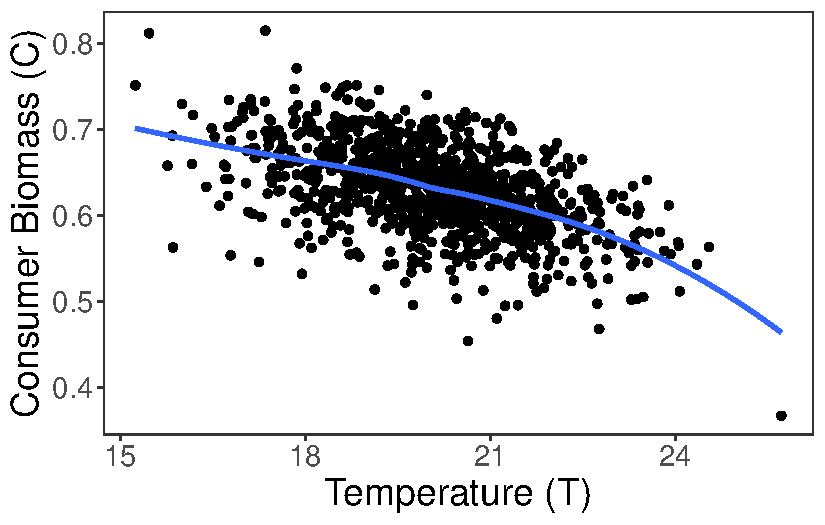
\includegraphics{index_files/figure-pdf/unnamed-chunk-2-1.pdf}

\begin{Shaded}
\begin{Highlighting}[]
\CommentTok{\# Plot the relationship between C and S}
\FunctionTok{ggplot}\NormalTok{(results, }\FunctionTok{aes}\NormalTok{(}\AttributeTok{x =}\NormalTok{ S, }\AttributeTok{y =}\NormalTok{ C)) }\SpecialCharTok{+}
    \FunctionTok{geom\_point}\NormalTok{() }\SpecialCharTok{+}
    \FunctionTok{geom\_smooth}\NormalTok{(}\AttributeTok{method =} \StringTok{"loess"}\NormalTok{, }\AttributeTok{se =} \ConstantTok{FALSE}\NormalTok{) }\SpecialCharTok{+}
    \FunctionTok{labs}\NormalTok{(}\AttributeTok{x =} \StringTok{"Resource Inflow (S)"}\NormalTok{, }\AttributeTok{y =} \StringTok{"Consumer Biomass (C)"}\NormalTok{) }\SpecialCharTok{+}
    \FunctionTok{theme\_bw}\NormalTok{() }\SpecialCharTok{+}
    \FunctionTok{theme}\NormalTok{(}
        \AttributeTok{text =} \FunctionTok{element\_text}\NormalTok{(}\AttributeTok{size =} \DecValTok{18}\NormalTok{),}
        \AttributeTok{panel.grid.major =} \FunctionTok{element\_blank}\NormalTok{(),}
        \AttributeTok{panel.grid.minor =} \FunctionTok{element\_blank}\NormalTok{(),}
        \AttributeTok{strip.background =} \FunctionTok{element\_blank}\NormalTok{()}
\NormalTok{    )}
\end{Highlighting}
\end{Shaded}

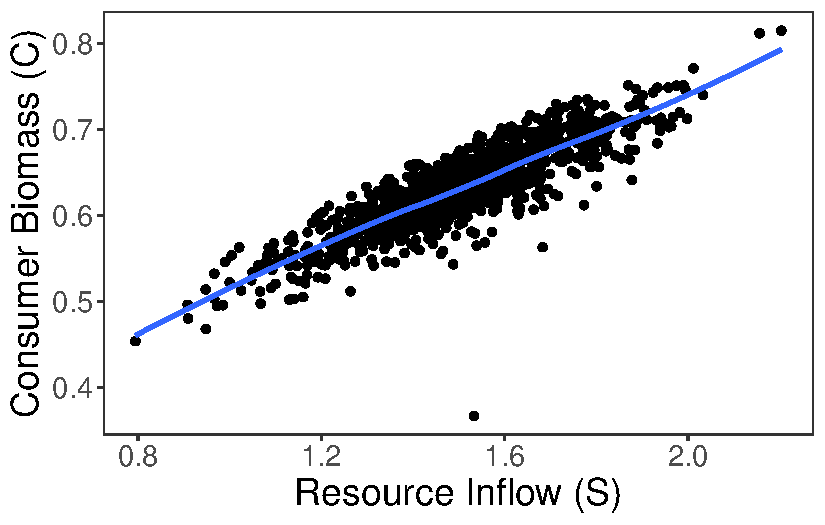
\includegraphics{index_files/figure-pdf/unnamed-chunk-2-2.pdf}

\begin{Shaded}
\begin{Highlighting}[]
\FunctionTok{ggplot}\NormalTok{(results)  }\SpecialCharTok{+} 
    \FunctionTok{geom\_histogram}\NormalTok{(}\FunctionTok{aes}\NormalTok{(}\AttributeTok{x =}\NormalTok{ C), }\AttributeTok{fill =} \StringTok{"blue"}\NormalTok{) }\SpecialCharTok{+} 
    \FunctionTok{theme\_bw}\NormalTok{() }\SpecialCharTok{+}
    \FunctionTok{theme}\NormalTok{(}
        \AttributeTok{text =} \FunctionTok{element\_text}\NormalTok{(}\AttributeTok{size =} \DecValTok{18}\NormalTok{),}
        \AttributeTok{panel.grid.major =} \FunctionTok{element\_blank}\NormalTok{(),}
        \AttributeTok{panel.grid.minor =} \FunctionTok{element\_blank}\NormalTok{(),}
        \AttributeTok{strip.background =} \FunctionTok{element\_blank}\NormalTok{()}
\NormalTok{    )}
\end{Highlighting}
\end{Shaded}

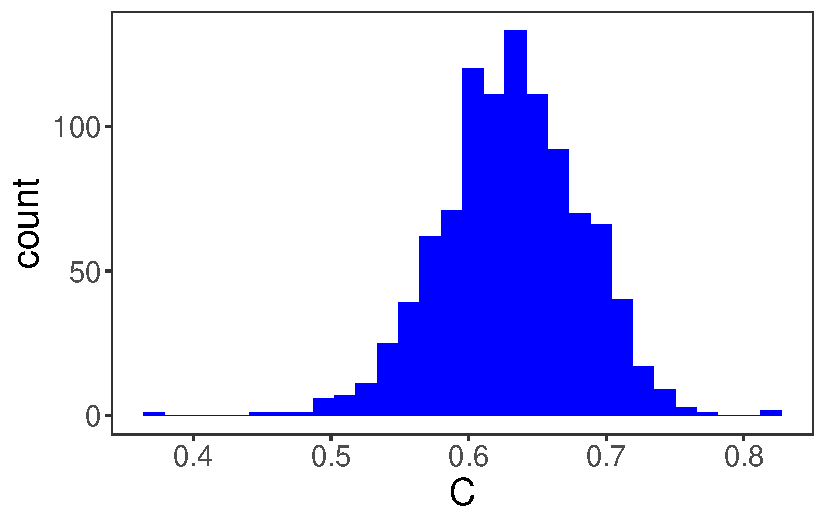
\includegraphics{index_files/figure-pdf/unnamed-chunk-2-3.pdf}

\begin{Shaded}
\begin{Highlighting}[]
\CommentTok{\# 3D plot of C with respect to both T and S}
\FunctionTok{scatter3D}\NormalTok{(}
    \AttributeTok{x =}\NormalTok{ results}\SpecialCharTok{$}\NormalTok{T, }\AttributeTok{y =}\NormalTok{ results}\SpecialCharTok{$}\NormalTok{S, }\AttributeTok{z =}\NormalTok{ results}\SpecialCharTok{$}\NormalTok{C,}
    \AttributeTok{pch =} \DecValTok{19}\NormalTok{, }\AttributeTok{cex =} \FloatTok{1.2}\NormalTok{, }\AttributeTok{colkey =} \ConstantTok{TRUE}\NormalTok{,}
    \AttributeTok{main =} \StringTok{"3D plot of C vs T and S"}\NormalTok{,}
    \AttributeTok{xlab =} \StringTok{"Temperature (T)"}\NormalTok{, }\AttributeTok{ylab =} \StringTok{"Resource Inflow (S)"}\NormalTok{, }
    \AttributeTok{zlab =} \StringTok{"Consumer Biomass (C)"}\NormalTok{,}
    \AttributeTok{theta =} \DecValTok{40}\NormalTok{, }\AttributeTok{phi =} \DecValTok{20}
\NormalTok{)}
\end{Highlighting}
\end{Shaded}

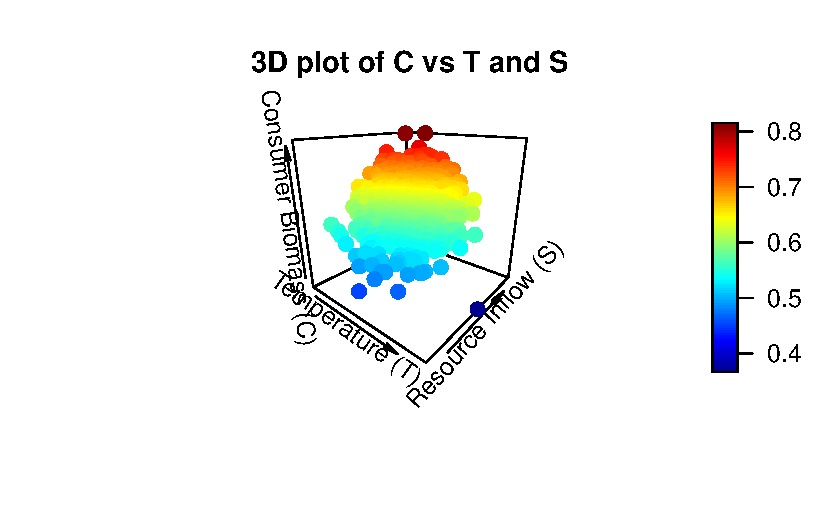
\includegraphics{index_files/figure-pdf/unnamed-chunk-2-4.pdf}

\begin{Shaded}
\begin{Highlighting}[]
\CommentTok{\# \# Create a 2D grid of T and S}
\CommentTok{\# plot\_matrix \textless{}{-} t(reshape2::acast(results, S\textasciitilde{}T, value.var="C"))}
\CommentTok{\# d\_df \textless{}{-} as.matrix(results[, c("C", "S", "T")], rownames.force = NA)}
\CommentTok{\# plot\_ly(z=\textasciitilde{}d\_df) \%\textgreater{}\% add\_surface()}

\CommentTok{\# plotly::plot\_ly(}
\CommentTok{\#       z=\textasciitilde{}d\_df}
\CommentTok{\#     ) \%\textgreater{}\% }
\CommentTok{\#   add\_surface() \%\textgreater{}\%}
\CommentTok{\#   layout(}
\CommentTok{\#     title = "",}
\CommentTok{\#     scene = list(}
\CommentTok{\#       xaxis = list(title = "S"),}
\CommentTok{\#       yaxis = list(title = "T"),}
\CommentTok{\#       zaxis = list(title = "C"),}
\CommentTok{\#       camera = list(eye = list(x = 1.95, y = {-}1.25, z = 1.25))}
\CommentTok{\#     ))}
\end{Highlighting}
\end{Shaded}

\textsubscript{Source:
\href{https://colebrookson.github.io/theRmal-landscape/index.qmd.html}{Article
Notebook}}

\phantomsection\label{refs}
\begin{CSLReferences}{1}{0}
\bibitem[\citeproctext]{ref-vintonResourceLimitationDetermines2022}
Vinton, Anna C., and David A. Vasseur. 2022. {``Resource Limitation
Determines Realized Thermal Performance of Consumers in Trophodynamic
Models.''} \emph{Ecology Letters} 25 (10): 2142--55.
\url{https://doi.org/10.1111/ele.14086}.

\end{CSLReferences}



\end{document}
